\documentclass[a4j,12pt]{jreport}
%\documentclass{jreport}
\usepackage[dvipdfmx]{graphicx}
% \usepackage[dvipdfmx]{graphics}
\usepackage{amsmath,amssymb}
% \usepackage{amsmath}
%\usepackage{pxjahyper}
\usepackage{here}
\usepackage{algorithm}
\usepackage{algpseudocode}
\usepackage{hhline}
\usepackage[hang,small,bf]{caption}
\usepackage[subrefformat=parens]{subcaption}
\usepackage{url}
\usepackage{mathrsfs}
\usepackage{amsmath}
\captionsetup{compatibility=false}

\def\syaji{ \chapter*{謝辞} \addcontentsline{toc}{chapter}{謝辞}}
\renewcommand{\bibname}{参考文献}
\setlength{\textheight}{\paperheight}
\setlength{\topmargin}{4.6mm}
\addtolength{\topmargin}{-\headheight}
\addtolength{\topmargin}{-\headsep}
\addtolength{\topmargin}{-\headheight}
\addtolength{\textheight}{-60mm}

\setlength{\textwidth}{\paperwidth}
\setlength{\oddsidemargin}{-0.4mm}
\setlength{\evensidemargin}{-0.4mm}
\addtolength{\textwidth}{-50mm}

\begin{document}

%%%%%%%%%%%%%%%%%%%%%
% 表紙
%%%%%%%%%%%%%%%%%%%%%
\thispagestyle{empty}
\begin{center}
\begin{Large}
\vspace*{0.7cm}
{\large 中央大学大学院理工学研究科情報工学専攻\\修士論文}\\
\vspace*{2.3cm}
{\bf 選挙区割問題に対するヒューリスティクスを用いた\\ZDD構築の効率化}\\
\vspace*{0.7cm}
{\sf Efficient ZDD Construction Using Heuristics \\for the Electoral Districting Problem}\\
\vspace*{5cm}
千原 良太\\
Ryota CHIHARA\\
学籍番号\hspace*{1zw}21N8100011I\\
\vspace*{2.5cm}
指導教員\hspace*{1zw} 今堀 慎治 教授\\
\vspace*{2.5cm}
2023年3月\\
\end{Large}
\end{center}


%%%%%%%%%%%%%%%%%%%%%
% 概要
%%%%%%%%%%%%%%%%%%%%%
\newpage
\renewcommand{\baselinestretch}{1.25} \selectfont
\pagenumbering{roman}


\begin{center} {\large \bf{概 要}} \end{center}

衆議院議員選挙小選挙区制における選挙区割問題とは,
各都道府県ごとに議席数(区割数)が定められており,
市区町村からなる小地域を組合せて区割を構成し,
その中から最も良い区割を見つける離散最適化問題の一種である.
実際の選挙区割では,人口の偏りによる「一票の格差」が問題提起されており,
人口の格差を最小にした区割の導出が求められている.

この問題の解法として,
ゼロサプレス型二分決定グラフ(ZDD)を用いた区割列挙が知られている.
区割数や各区割の人口の上限・下限などを制約として与え,その制約から枝刈りを行うことで,
解候補を列挙することができる.
ただし,区割人口の上下限制約は,平均人口から一律に定められた格差許容定数を用いて計算し,
メモリ不足等で解が導出できない場合のみ値を変更する手法が多く取られていた.

本論文では,ヒューリスティクスを用いて人口の上下限制約を定め,
それを基にZDDを構築することで,
従来よりも効率的に解候補を得る手法を提案する.
また,計算機実験を行い,
従来手法よりもZDD構築における計算時間とメモリ消費量が削減できることを確認する.


\vspace{1zw} \noindent
{\bf キーワード: }離散最適化,選挙区割問題,ZDD,ヒューリスティクス.

%%%%%%%%%%%%%%%%%%%%%
% 目次
%%%%%%%%%%%%%%%%%%%%%
\tableofcontents


\newpage
\pagenumbering{arabic}

%%%%%%%%%%%%%%%%%%%%%
% 本文
%%%%%%%%%%%%%%%%%%%%%
%%%%%%%%%%%%%%%%%%%%%
% 1章
%%%%%%%%%%%%%%%%%%%%%
\chapter{はじめに} \label{chapter:1}
日本の衆議院議員選挙における小選挙区制の区割は,
総定数から各都道府県に何議席を割り当てるかを決める定数配分問題と
都道府県内で,割り当てられた議席数分の選挙区を市区町村を組合せて構築する
区割画定問題を解くことによって,定めることができる.

定数配分問題は,法学,公共政策学,数理情報学などの様々な観点から
取り組まれており,過去200年以上にわたり多くの手法が提案されている.
2022年12月28日には,公職選挙法の一部を改正する法律(区割り改定法)が施行され,
衆議院小選挙区選出議員の選挙区について「アダムズ方式」を用いた議席の配分が行われた\cite{ichimori}.
アダムズ方式はアメリカ6代目大統領ジョン・アダムズが考案したとされており,
簡単に説明すると
「各都道府県の人口をある自然数で割った商の小数点以下を切り上げた数を,
その都道府県の議席数とする」手法である.
この手法は,一票の格差の是正には効果的とされているが,
「アラバマ・パラドックス」と呼ばれる改訂時に議席総数が増加した際に,
ある地区では配分される議席数が改訂前より減る現象が起こる場合がある.
また,過去に提案された手法を比較したときに,一票の格差がほぼ等しい場合でも,
各都道府県の人口が多い方が有利な手法,少ない方が有利な手法といった
差が現れ,どの手法も一長一短であることから,
選挙制度の意義等も踏まえつつ議論する必要がある.
本稿では,定数配分問題については主に扱わず,2021年に行われた第49回衆議院議員選挙の
定数配分をそのまま利用する.

区割画定問題は,都道府県内の選挙区の組合せが市区町村数の指数通り存在し,
NP困難であるとして,20世紀末までは最適性の保障のない解の導出の研究が主であった.
しかし,2003年に根本・堀田が数理モデルによる定式化を提案\cite{nemoto}して以降,
数理的な観点から多くの研究が取り組まれており,
厳密解を導出するための手法がいくつか提案されている.
その中の手法の一つとして,ゼロサプレス型二分決定木(ZDD)を用いた
区割列挙があり,フロンティア法によってトップダウンにZDDを構築することで,
高速に選挙区割を求めることが可能となっている.
ただし,いくつかの都道府県においては計算機のメモリ不足により解を導出することが
困難である.

本研究では,区割画定問題(以下「選挙区割問題」と称する)における
ZDDを用いた区割列挙について扱い,
ヒューリスティクスを用いて効率的に区割列挙を行う手法を提案する.
本稿の第2章では選挙区割問題について定義し,
数理モデルによる定式化を説明する.
第3章ではZDDとフロンティア法,
それを用いた区割列挙アルゴリズムについて詳しく述べる.
第4章では,第3章で説明したアルゴリズムとヒューリスティクスを組合せることで
ZDD構築を効率化する手法を提案する.
そして,第5章で計算機実験の結果とその考察を示し,
第6章で結論と今後の課題について述べる.

%%%%%%%%%%%%%%%%%%%%%
% 2章
%%%%%%%%%%%%%%%%%%%%%
\chapter{選挙区割問題} \label{chapter:2}

本章では,選挙区割問題について,国の公表資料から区割作成方針を示し,
問題の定義,数理モデルによる定式化について説明する.

\section{区割作成方針}
衆議院議員選挙の選挙区割の改定案は,
衆議院議員選挙区画定審議会によって作成される.
当審議会では,令和4年2月21日に『区割り改定案の作成方針』を公表しており,
作成方針を簡潔に述べると以下の6点となる.
\begin{enumerate}
    \item 一票の格差は2倍未満とする.
    \item 議員1人当たり人口が最も少ない県においては,各選挙区の人口をできるだけ均等にする.
    \item 改定案の作成にあたり,選挙区の区域の異動は,
    区割り基準に適合させるために必要な範囲とする.
    \item 選挙区は飛び地にしない.
    \item 選挙区を構成する市区町村は原則分割しない.
    \item 地勢,交通,人口動向などの自然的,社会的条件を総合的に考慮する.
\end{enumerate}

本研究では,項目1,2,4,5を主に考慮する.
ただし,項目2は,人口最小の県だけでなく,
全ての都道府県において各選挙区の人口をできるだけ均等にすることを目指す.
項目3は,改定前との区割の比較が研究の主旨ではないため考慮しない.
項目6は,モデル化するには複雑であるため,今回は飛び地にしないことで,
自然的,社会的条件を満たしているとみなす.

\section{問題定義}

区割作成方針をもとに問題を定義する.
まず,都道府県ごとに市区町村とその隣接関係,
各市区町村の人口を重みつきグラフ$G=(V, E, w)$で表現する.
入力は,市区町村数を$l$として,市区町村集合$V=\{v_1,...,v_l\}$, 
市区町村の隣接関係$E=\{\{v_i,v_j\}|$市区町村$v_i$と$v_j$は隣接$\}$, 
市区町村$v_i$の人口$w_i$,選挙区数$d(<l)$が与えられる.
そして出力は,$d$個の選挙区の集合$S=(S_1,...,S_d)$であり,
$S_k$は$k$番目の選挙区に属する市区町村の集合を表す.
ただし,選挙区は以下の制約を満たす必要がある.\\
\quad\textbf{制約1}:選挙区に属する市区町村から誘導される部分グラフは連結である.\\
\quad\textbf{制約2}:全ての市区町村は唯一つの選挙区に属す.\\
\quad\textbf{制約3}:選挙区は空集合ではない.

また,選挙区ごとの人口の和$P=\{P_1,...,P_d\}$ ($P_k=\sum_{v_i\in S_k}w_i\ (k=1,...,d)$)を計算し,
選挙区人口の最小値$\mathrm{min}(P)$ と最大値$\mathrm{max}(P)$を調べる.
制約を満たす選挙区割の中で,一票の格差が最小のもの,
すなわち$\frac{\mathrm{max}(P)}{\mathrm{min}(P)}$の値が最小であるものを最適な選挙区割と定める.


\section{モデル表現}
選挙区割を表す数理モデルの代表例として,集合分割型モデル\cite{nemoto}を説明する.
まず,制約1から連結である市区町村の集合をブロックと名付ける.
空集合を除く全てのブロック集合を$\mathscr{B}$で表し,
ブロック集合$\mathscr{B}$から選んだ$d$個のブロックが制約2を満たすと,
実行可能な区割となる.その中で一票の格差が最小な区割を見つける.

\textbf{入力データ}:市区町村集合$V$,選挙区数$d$,
ブロック集合$\mathscr{B}$を表す行列$[b_{ij}|i=1,...,n,~j=1,...,|\mathscr{B}|]$:
市区町村$v_i$がブロック$j$の構成要素のとき$b_{ij}=1$;
そうでないとき$b_{ij}=0$,
ブロック$j$の人口$q_j=\sum_{i\in n}b_{ij}w_{i}~(j=1,...,|\mathscr{B}|)$.

\textbf{変数}:一つの選挙区の人口上限を示す変数$u$,下限を示す変数$l$,
バイナリ変数$x_j~(j=1,...,|\mathscr{B}|)$:
区割にブロック$j$を使用するとき$x_j=1$;しないとき$x_j=0$.

\textbf{定式化}:
\begin{align}
    &\mathrm{minimize} && u/l && \\
    &\mathrm{subject~to} && q_jx_j\leq u~~(j=1,...,|\mathscr{B}|) && \\
    & && \alpha(1-x_j)+q_jx_j\geq l~~(j=1,...,|\mathscr{B}|) && \\
    & && \sum_{j=1,...,|\mathscr{B}|}b_{ij}x_{j}=1~~(i = 1, ... , n) && \\
    & && \sum_{j=1,...,|\mathscr{B}|}x_j=d && \\
    & && x_j \in \{0,1\}~~(j=1,...,|\mathscr{B}|) &&
\end{align}

ここで,$\alpha$は十分大きな定数とする.
式(2.1)は一票の格差を最小化することを目的関数として示している.
式(2.2)と(2.3)は変数$u$と$l$を正しく表すために必要な制約である.
式(2.4),(2.5),(2.6)は制約2を表現している.
また,制約1と3についてはブロック集合$\mathscr{B}$から選挙区を構成しているため,
条件を満たしている.よって,上述の形で選挙区割問題を定式化することができる,
%%%%%%%%%%%%%%%%%%%%%
% 3章
%%%%%%%%%%%%%%%%%%%%%
\chapter{ZDDを用いた区割列挙手法} \label{chapter:3}

\section{概要}

\section{ゼロサプレス型二分決定グラフ}

\section{フロンティア法}

\section{区割列挙アルゴリズム}

\subsection{人口制約なしの場合}

\subsection{人口制約ありの場合}

%%%%%%%%%%%%%%%%%%%%%
% 4章
%%%%%%%%%%%%%%%%%%%%%
\chapter{ヒューリスティクスを用いた手法} \label{chapter:4}

本章では,選挙区割問題を解くヒューリスティクスを作り,
その解から得られた選挙区の人口上限と下限を用いて,
ZDD構築を効率化する手法について提案する.

\section{概要}

\ref{chapter:3}章の人口制約付きZDD構築アルゴリズムでは,
パラメータとして部分グラフの重み上限$U$,下限$L$を用いた.
これを,許容格差定数$r$を使わず,ヒューリスティクスの解から,
最適解にできるだけ近い$U$,$L$を定義する.
$U$,$L$が最適解に近くなればなるほど,ZDDの構築時に,
最適解でない解候補の枝刈りの回数が多くなる.
その結果,従来手法に比べて
メモリの使用量の減少及び計算時間の短縮が期待できる.
提案手法の全体像を図\ref{heuristics}に記した.

\begin{figure}[htbp]
  \centering
  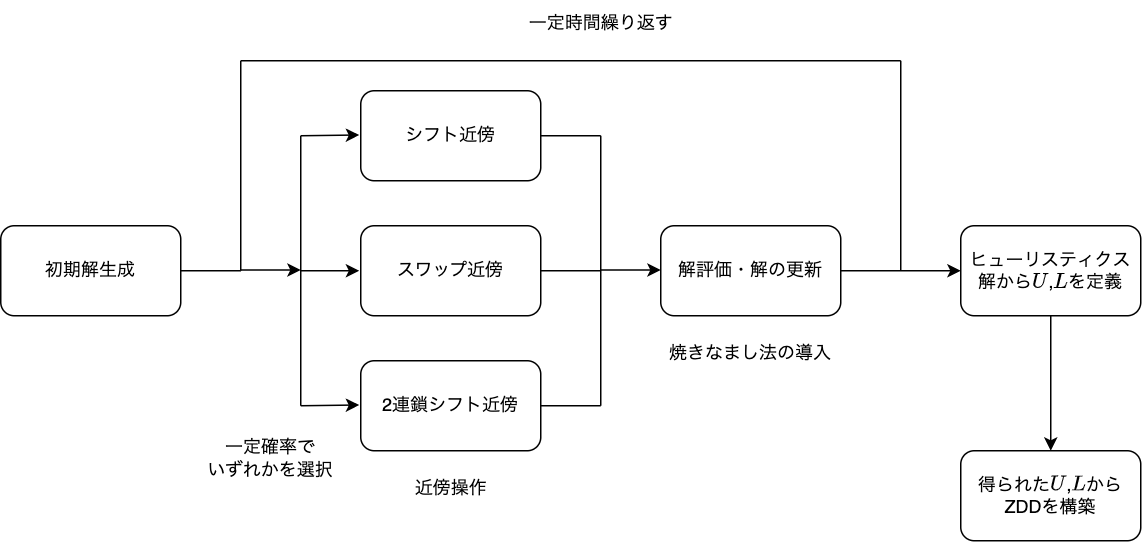
\includegraphics[scale=0.39]{img/heuristics.png}
  \caption{ヒューリスティクスを用いた提案手法}
  \label{heuristics}
\end{figure}



\section{初期解生成}

初期解は,幅優先探索を

\section{近傍操作}

\subsection{シフト近傍}

\begin{figure}[htbp]
  \centering
  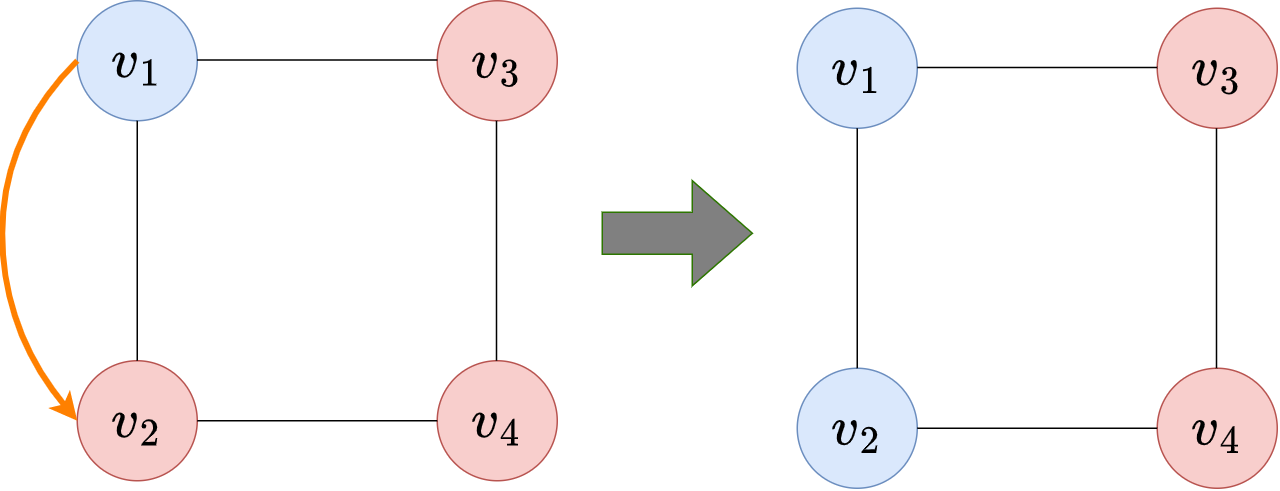
\includegraphics[scale=0.2]{img/shift-neighbor.png}
  \caption{シフト近傍}
  \label{shift-neighbor}
\end{figure}

\subsection{スワップ近傍}

\begin{figure}[htbp]
  \centering
  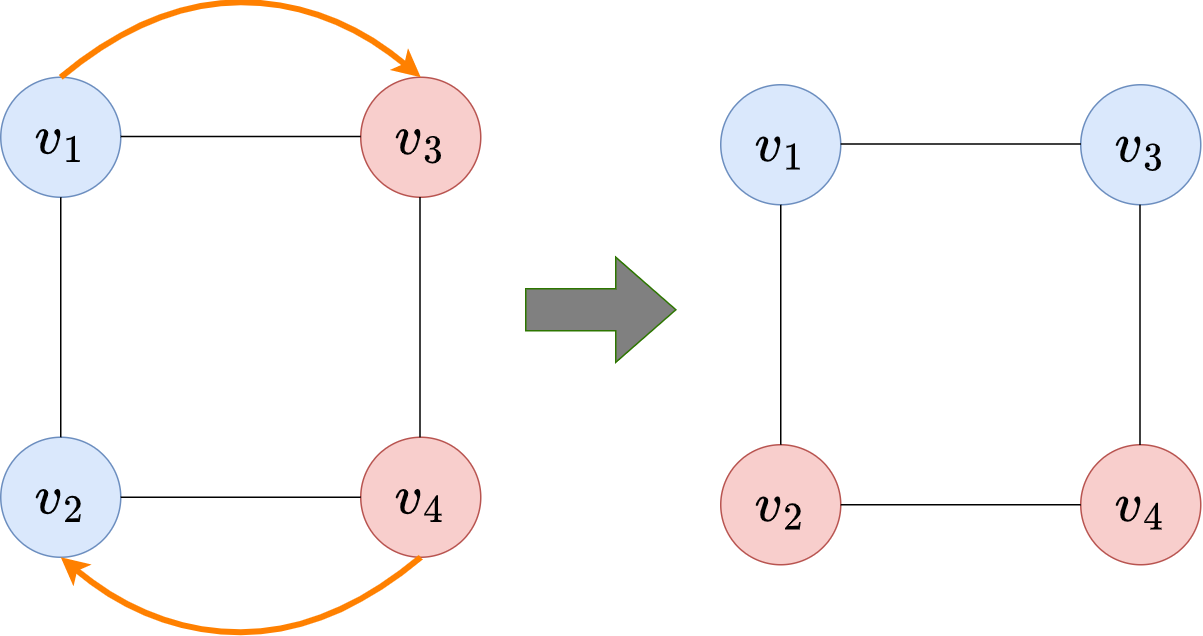
\includegraphics[scale=0.2]{img/swap-neighbor.png}
  \caption{スワップ近傍}
  \label{swap-neighbor}
\end{figure}

\subsection{2連鎖シフト近傍}

\begin{figure}[htbp]
  \centering
  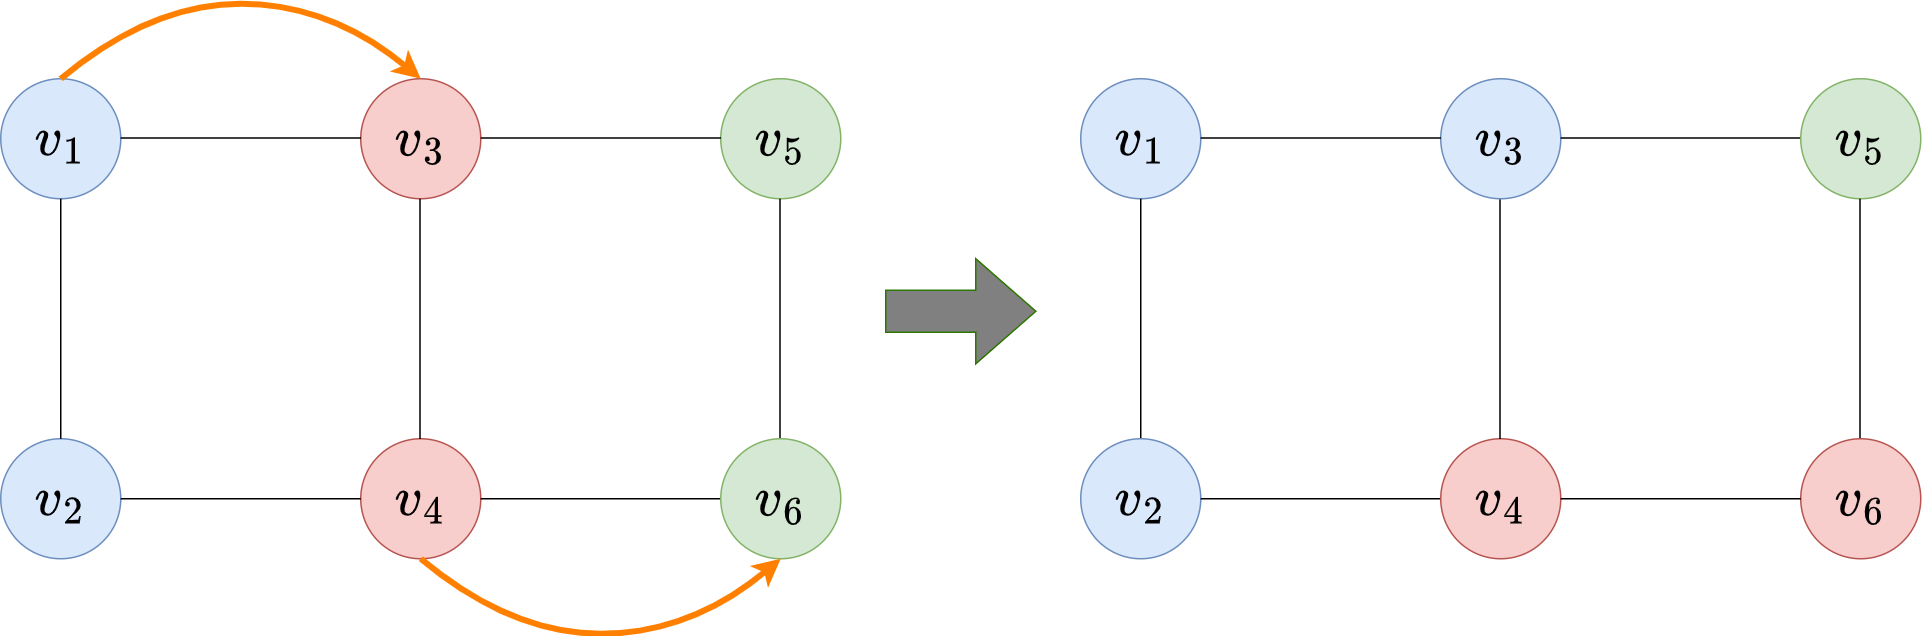
\includegraphics[scale=0.2]{img/chain-neighbor.png}
  \caption{2連鎖シフト近傍}
  \label{chain-neighbor}
\end{figure}

\section{焼きなまし法}


%%%%%%%%%%%%%%%%%%%%%
% 5章
%%%%%%%%%%%%%%%%%%%%%
\chapter{計算機実験} \label{chapter:5}

\section{概要}

\section{実験環境}

\section{入力データ}

\section{実験結果}

\subsection{人口制約なし}

\subsection{人口制約あり:格差許容定数を用いる場合}

\subsection{人口制約あり:ヒューリスティクスの結果を用いる場合}

\section{考察}
%%%%%%%%%%%%%%%%%%%%%
% 6章
%%%%%%%%%%%%%%%%%%%%%
\chapter{計算機実験} \label{chapter:6}


%謝辞
\syaji
\par
本研究を進めるにあたり,大変多くのご指導,ご助言を頂いた
中央大学理工学部情報工学科の中央太郎教授に深く感謝いたします.
また,多大なるご助言,ご協力を頂いた〇〇研究室の皆様には大変お世話になりました.
心から感謝いたします.


%参考文献
\begin{thebibliography}{99}
\addcontentsline{toc}{chapter}{参考文献}

\bibitem{ichimori}
一森哲夫:議席配分の数理-選挙制度に潜む200年の数学-,近代科学社(2022).

\bibitem{nemoto}
根本俊男,堀田敬介:区割画定問題のモデル化と最適区割の導出,オペレーションズ・リサーチ,
vol.~48,no.~4,pp.~300-306(2003).

\bibitem{suetake}
末武国弘,科学論文をどう書くか,講談社ブルーバックス,講談社,東京,1981.

\bibitem{kusano}
草野花子,中大太郎,パラメトリック増幅器,電子情報通信学会論文誌,vol.~J62-B, no.~1, pp.~20--27, 1979. 

\bibitem{fuortes}
M. G. F. Fuortes, ed., \textit{Handbook of Sensory Physiology}, Springer-Verlag, Berlin, 1972.

\bibitem{rice}
W. Rice, A. C. Wine, and B. D. Grain, Diffusion of impurities during epitaxy, \textit{Proc. IEEE}, vol.~52, no.~3, pp.~284--290, 1964.

\bibitem{guibas}
L. J. Guibas and R. Sedgewick, A dichromatic framework for balanced trees, 
\textit{Proc. 19th IEEE Sympos. Found. Comput. Sci.}, Ann Arbor, pp.~8--21, 1978.

\bibitem{chudai}
中大次郎,マルチメディアと数理工学,中央大学大学院理工学研究科情報工学専攻修士論文,1998.

\bibitem{iwama}
K. Iwama, A. Kawachi, and S. Yamashita, Quantum biased oracles, \textit{IPSJ Digital Courier}, vol.~1, pp.~461--469 (online), DOI: 10.2197/ipsjdc.1.461, 2005.

\bibitem{IPSJ}
情報処理学会,論文誌ジャーナル(IPSJ Journal)原稿執筆案内,情報処理学会(オンライン),入手先〈\url{https://www.ipsj.or.jp/journal/submit/ronbun_j_prms.html}〉(参照2022-04-25).


\end{thebibliography}

%関連論文, 仕様はthebibliographyと同一. 
%\begin{therelatedreference}{99}
%\end{therelatedreference}

\end{document}